\chapter{User interface}\label{chap:ui}

\section{UI}
This chapter concerns building an application providing a user interface to the
pan-tilt system. The application runs on the ARM Cortex M3 based EMP-board
(Reference ???)

\subsection{Requirements}
The UI must allow the user to see a numerical expression
describing the position of the system. The user must also be able to set the
wanted position of the system, either by entering the wanted values, or by
recording multiple positions and shifting between them.

It should also be considered making a simple solution where the potmeter
controls the pan and the digiswitch controls the tilt to provide some kind of
realtime control.

The main application for the UI will be in testing the pan-tilt system.
Therefore a logging system must be built to provide data for the development
and testing of the system. It is not definite which numbers and values are
interesting, so a versatile and easily adaptable system is required.

Though the system will be used mainly by people with some programming
experience, it must provide an easy way of configuring and altering the functionalities of the system. Since it is a faily complex system it should be separated and organized to ensure as little focus on programming as possible while configuring and testing the system.

The  menu structure displayed in figure \ref{fig:menu_structure} must be implemented ...

\begin{figure}[htb]
	\centering
	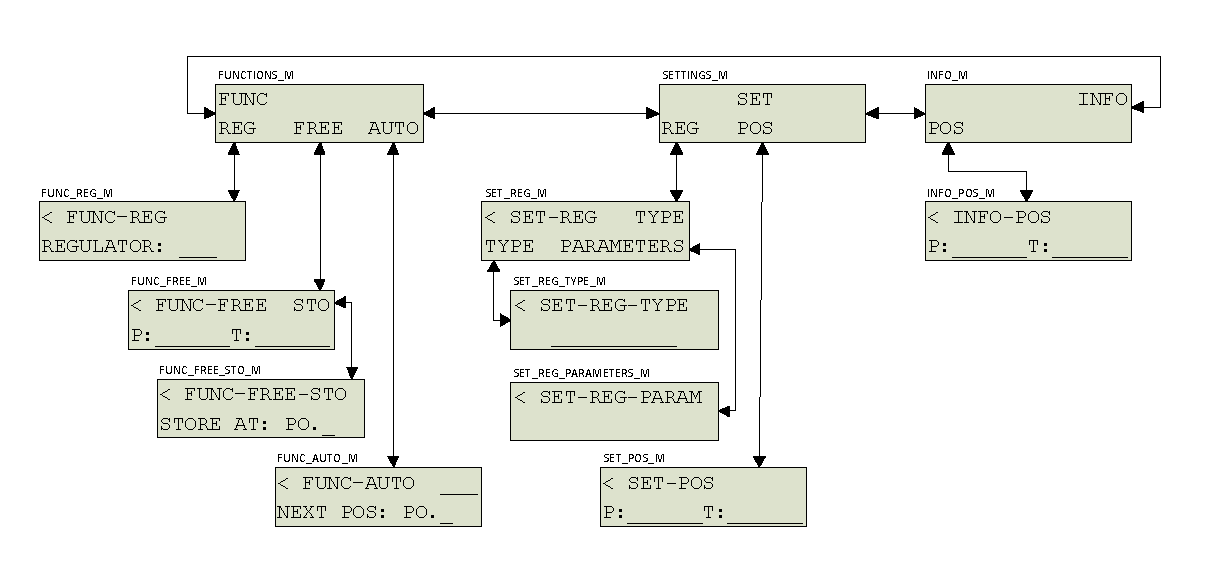
\includegraphics[scale=1,trim=0 0 0 0]{graphics/menu_structure.pdf} 
	\caption{Structure of the menu system}
	\label{fig:ui_task_diagram}
\end{figure}

\subsection{Discussion}
The EMP-board provides several channels for outputting data to the user. One is
by communication to a computer terminal. This is a good way of displaying large
amount of data, but should be kept in simple ASCII based text format. It is
important to provide a simple interface so output can be easily changed.

Another output channel is the two displays. Since focus is on displaying facts
rather than graphics, the small LCD display should not be used. Since the 16x2
is limited to displaying 32 characters at any time, it is necessary to implement
some form of menu system.
 
The EMP board also provides a number of inputs. There are several buttons, but
given the easy to use requirements the use of buttons is avoided. That leaves
the digiswitch as the main input to control the menus and the potentiometer as a
secondary input.



\subsection{Implementation}
Implementing a menu based state machine can be split into two parts. One
concerns the user navigating the menus and the other concerns having the menus or inputs to them
control the rest of the system. 

To make the system easy to reconfigure, the menus and their functionalities are based uponthe configuration file menu\_setup.c. A menu concists of two lines of menu text and a number of fields to shuffle through using the dreh impuls geber. 

The menu task has the responsibility of handling the systems inputs and outputs based on the rules given by the menu items. Normally it would be preferred to have the task block on a queue or a semaphore, but in this case since there are two types of input to be handled another approach is needed.  Input from the user and updated values from the SPI connection must both be handled by the menu task, but the updates come at fixed intervals at all times and the user inputs are events happening at random times.

Normally it would be preferred to split the task into two sub tasks, each responsible for their own input and thus differently timed. If this approach was followed, the menu task would be split into an input handling task and an output handling task and the output task would run every time the parameters had been updated. 

The reason for the frequent updates is to provide accurate data for the control algorithm, but there is no need to update the display this often. This is he reason for not dividing the menu task. Instead the task runs every five milliseconds, which is sufficient to service both inputs and outputs without the user noticing any delays. Some operating systems support blocking on multiple conditions, but this is not supported by FreeRTOS so on this system blocking on time is the best solution.

\subsection{Task diagram}
Layers....

The menu task first handles inputs from the dreh impuls geber and updates current menu based on this. It then checks whether any of the fields in the current menu takes input and handles theese updating relevant parameters. Then the display buffer is updated to contain the two lines provided by the current menu and data from any output fields are written to the buffer before yielding. The system state is held entirely in the menu item, thus reducing the menu task to a piece of sequential code.

\begin{figure}[htb]
	\centering
	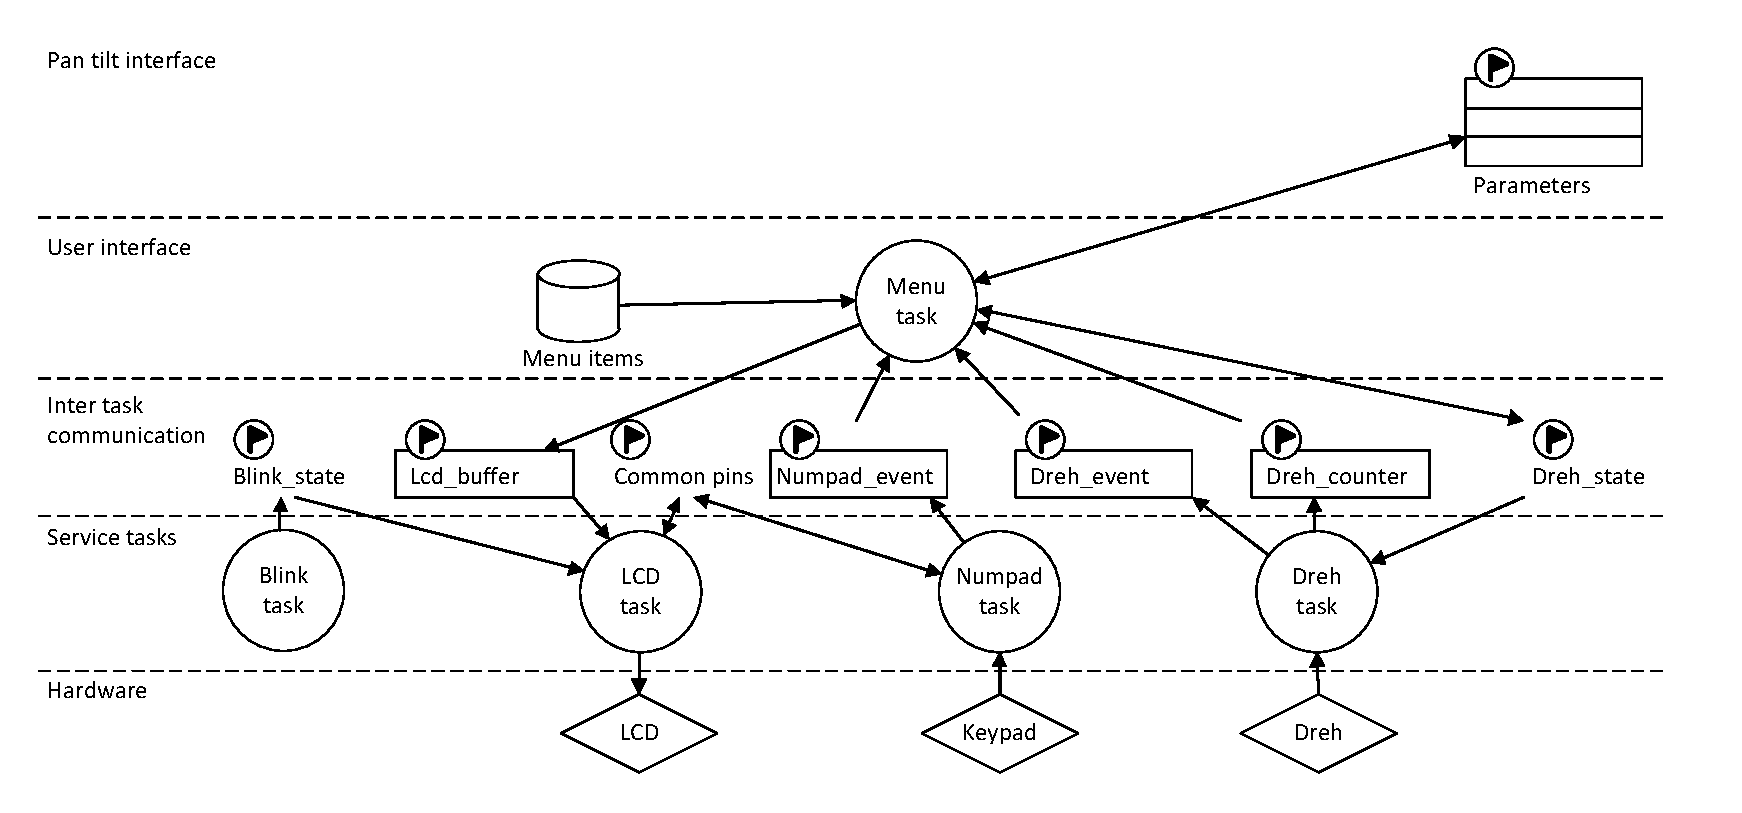
\includegraphics[scale=1,trim=0 0 0 0]{graphics/task_diagram_user_interface.pdf} 
	\caption{Task diagram for the user interface}
	\label{fig:ui_task_diagram}
\end{figure}

The menus are implemented as a linked list to make it possible to add menus from a serial connection or from the user interface. Position setpoints ca then be implemented as menu point to make it possible to cycle through any number of user defined positions in any order.

The linked list is accessed through the menu handler interface that allocates the position data dynamically and passes as a pointer to the position.

\section{Service tasks}
The peripherals provided by the EMP board are each assigned a service task. Theese tasks are based on code developed during the EMP course though some changes had to be made in order to comply with a preemptive system. 

\subsection{Lcd task}
The lcd task works on a mutex protected buffer and simply runs through the buffer checking the dirty bit and the blink bit of every character in the buffer. If the dirty bit is set, the corresponding character on the lcd display is updated. If the blink bit is set and the blink state is active, the preset blink character is displayed instead of the buffer character.

\subsection{Dreh task}
The dreh impuls geber also known as a digiswitch is an electrical component that outputs a pair of phase shifted pulse trains when turned. The pulses are used to determine the turning direction as well as the number of clicks. The rod on the dreh impuls geber can also be pushed and thus functions like any button.

The driver software for the dreh impuls geber is based on a finite state machine shown in fig XXX. When run the task compares the current state of the three input pins with the saved states. If there are differences, it generates an event based on the pins.

\subsection{Numpad task}
The numpad is a three by four matrix wired so that horisontal lines can be powered so that a pushed button will close a connection and thus the state of the four pins connected to the vertical lines will read high if pressed an low otherwise.

Since the numpad and lcd display share some common pins theese pins are protected by a mutual exclusion.

Numpad task is based on a Mealy finite state machine, following the diagram in figure XXX.  Some flicker was experienced and thus a flicker catch was implemented to delay the chance of state until thirty consecutive tests have confirmed the release of the button.

\subsection{Blink task}
The blink task controls the blinking characters on the display and is implemented as a Moore finite state machine. It runs every 350 milliseconds and changes the state according to the previous state. The state machine diagram in\ref{fig:blink_fsm_diagram} shows the transition between the on and off states.

\subsection{Tuning the tasks}
The tasks were all implemented as yielding tasks with idle priority, since none of them are time critical. Yield time of the tasks can be seen in table \ref{tab:ui_task_timing}.

\begin{table}[htb]	
	\begin{center}
	\begin{tabular}{l|l}					
	Task & Period \\					
	\hline							
LCD task & 2 ms \\
Dreh task  & 10 ms \\
Numpad task & 40 ms \\
Menu task & 80 ms \\
Blink task & 350 ms \\
	\end{tabular}
	\end{center}
	\caption{Timing of the user interface tasks}	
	\label{tab:ui_task_timing}				
\end{table}





















